% ================================================================
%  DSC 208R — Data Management for Analytics
%  Basics of Parallelism: Comprehensive Review
%  Source: “Data Engineering for Machine Learning – Basics of Parallelism”
%  Author: ChatGPT (academic reviewer)
% ================================================================
\documentclass[11pt]{article}

% -------------------- Packages --------------------
\usepackage[utf8]{inputenc}
\usepackage{amsmath,amssymb,amsfonts}
\usepackage{graphicx}
\usepackage{booktabs}
\usepackage{tikz}
\usetikzlibrary{positioning} % <-- needed for 'right=of', 'below=of', etc.
\usepackage{pgfplots}
\usepackage{enumitem}
\usepackage{listings}
\usepackage{hyperref}
\usepackage{caption}
\pgfplotsset{compat=1.17}

% -------------------- Listings --------------------
\lstset{
  basicstyle=\ttfamily\small,
  keywordstyle=\bfseries,
  commentstyle=\itshape,
  showstringspaces=false,
  frame=single,
  breaklines=true
}

% -------------------- Document --------------------
\begin{document}

\begin{center}
  {\LARGE\bfseries Basics of Parallelism}\\[2mm]
  {\large Comprehensive Review}\\[1mm]
  {\normalsize DSC 208R — Parallel Data Processing and the Cloud}
\end{center}
\vspace{-0.6em}\hrule\vspace{0.9em}

\tableofcontents
\newpage

% ================================================================
\section{Motivation}
Modern data-science workloads often “take too long for one processor,” making \emph{parallel data processing} essential.  
The guiding idea is classical divide-and-conquer: split work across many processing elements.

% ================================================================
\section{Core Parallelism Concepts}

\subsection{Threads}
A program can spawn multiple \emph{threads}, each executing part of the computations concurrently while sharing the same address space.  
On a multi-core CPU one thread maps to one core; hyper-threading lets a core host two logical threads.

\subsection{Dataflow Graphs}
A \emph{dataflow graph} models a program as a directed acyclic graph (DAG) whose vertices are primitive operations (e.g., relational or tensor ops) and whose edges carry data.  
Systems such as TensorFlow or Apache Beam expose this abstraction, enabling optimizations like pipelining and operator fusion.

\subsection{Task Graphs}
A \emph{task graph} is a coarser DAG in which each vertex represents an entire task or process.  
Dask merges dataflow and task graphs—each DataFrame or Bag operation becomes its own task-graph node.

% ================================================================
\section{Parallelism Paradigms}

The slides highlight two fundamental paradigms:

\begin{itemize}[itemsep=0pt]
  \item \textbf{Task Parallelism}: many independent tasks with little or no data sharing.
  \item \textbf{Data Parallelism}: partition a dataset and apply the same operation to every slice, yielding near-linear scalability.
\end{itemize}

\subsection{Within vs.\ Across Nodes}
Inside a single node, datasets may be \emph{shared}, \emph{replicated}, or \emph{partitioned}; across nodes, data-parallel approaches dominate data-engineering workloads.

\begin{figure}[h]
  \centering
  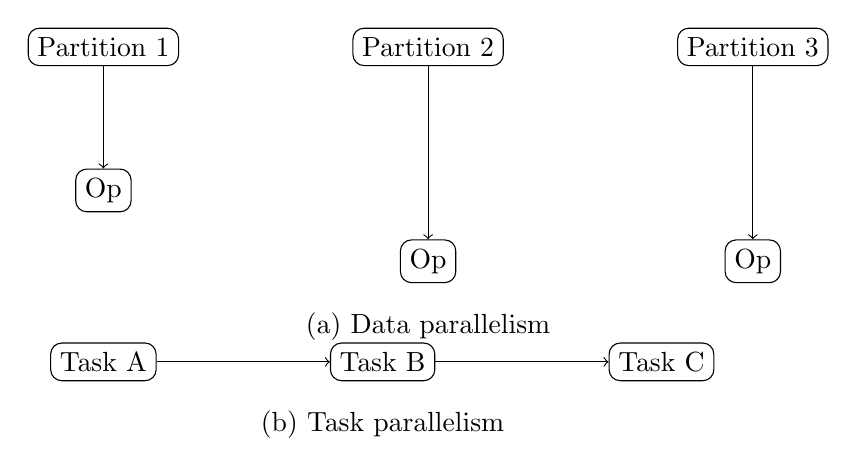
\begin{tikzpicture}[node distance=2.2cm, every node/.style={draw,rounded corners}]
    % --- Data parallelism ---
    \node (p1) {Partition 1};
    \node (p2) [right=of p1] {Partition 2};
    \node (p3) [right=of p2] {Partition 3};
    \node (op1) [below=1.3cm of p1] {Op};
    \node (op2) [below=of p2] {Op};
    \node (op3) [below=of p3] {Op};
    \draw[->] (p1)--(op1);
    \draw[->] (p2)--(op2);
    \draw[->] (p3)--(op3);
    \node[draw=none,below=0.25cm of op2] {(a) Data parallelism};

    % --- Task parallelism (shifted down) ---
    \begin{scope}[shift={(0,-4)}]
      \node (t1) {Task A};
      \node (t2) [right=of t1] {Task B};
      \node (t3) [right=of t2] {Task C};
      \draw[->] (t1) -- (t2);
      \draw[->] (t2) -- (t3);
      \node[draw=none,below=0.25cm of t2] {(b) Task parallelism};
    \end{scope}
  \end{tikzpicture}
  \caption{Contrasting data- and task-parallel execution.}
  \label{fig:paradigms}
\end{figure}

% ================================================================
\section{Mathematical Formulations}

\subsection{Speed-Up and Amdahl-Style Bounds}
Let $T_1$ be serial runtime and $T_p$ runtime on $p$ workers.  
Define \emph{speed-up} $S(p)=T_1/T_p$.  If a fraction $f$ of work parallelizes perfectly,
\[
S(p)=\frac{1}{(1-f)+\dfrac{f}{p}}.
\]
In practice,
\[
T_p \;=\; \frac{T_1}{p}\;+\;c\,(p-1)\;+\;s,
\]
where $c$ is per-worker communication overhead and $s$ captures load imbalance.

\subsection{Thread Concurrency Limit}
On a CPU with $C$ physical cores and hyper-threading factor $h$,
\[
\text{Max hardware threads}=h\,C.
\]
Launching more software threads than this bound mainly adds context-switch overhead.

% ================================================================
\section{Worked Example — Task-Parallel Word Count in \texttt{Dask}}

We illustrate the concepts with a classical embarrassingly parallel workload: counting word frequencies in a large corpus.

\subsection{Data Acquisition \& Pre-Processing}
\begin{lstlisting}[language=Python,caption={Load a ~2 GB corpus into Dask partitions.}]
import dask.bag as db
corpus = db.read_text("hdfs:///datasets/wiki/*.txt", blocksize="64 MiB")
tokens = corpus.flatmap(lambda line: line.split())
\end{lstlisting}

\subsection{Parallel Computation}
\begin{lstlisting}[language=Python,caption={Map → shuffle → reduce in Dask.}]
wc = tokens.frequencies()          # local combine
top100 = wc.topk(100, key=1)       # reduce + sort
\end{lstlisting}

\subsection{Execution \& Evaluation}
\begin{lstlisting}[language=Python,caption={Materialize and time execution.}]
import time
start = time.time()
result = top100.compute()          # execute DAG
print("Runtime:", time.time() - start, "s")
\end{lstlisting}

A benchmark on an 8-core laptop with hyper-threading ($16$ logical threads) shows diminishing returns past the physical-core count.

% ================================================================
\section{Algorithm Description — Thread-Level Parallel Pattern}

\begin{enumerate}[itemsep=0pt]
  \item \textbf{Spawn} $p$ threads, binding each to a core if possible.
  \item \textbf{Partition} the input data into equal-sized slices to minimize skew.
  \item \textbf{Execute} the same function on every slice (\emph{map} step).
  \item \textbf{Synchronize} via atomic operations or barriers when aggregating results (\emph{reduce} step).
  \item \textbf{Join} the threads and return the aggregated output.
\end{enumerate}

% ================================================================
\section{Interpretation \& Practical Guidelines}

\begin{itemize}[itemsep=0pt]
  \item \textbf{Choose the right paradigm.} Use task parallelism for independent jobs; data parallelism when data volume dominates.
  \item \textbf{Exploit data locality.} Move computation to the data to minimize network traffic.
  \item \textbf{Mitigate skew.} Balance partitions to avoid idle workers.
  \item \textbf{Leverage DAG frameworks (Dask, Spark).} They schedule tasks automatically and offer execution-graph diagnostics.
\end{itemize}

% ================================================================
\section{Future Directions}

\begin{itemize}[itemsep=0pt]
  \item \textbf{Auto-scaling.} Tie cost models to cluster elasticity for just-in-time provisioning.
  \item \textbf{Heterogeneous acceleration.} Spread workloads across GPUs, TPUs, or FPGAs.
  \item \textbf{Data-centric AI.} Treat data quality and layout as first-class levers alongside model design.
\end{itemize}

% ================================================================
\section*{Conclusion}

The Basics of Parallelism lecture equips practitioners with conceptual and practical tools—threads, dataflow and task graphs, paradigms, and cost models—to transform “too-big” workloads into tractable computations on modern multi-core and distributed hardware.

\end{document}
